\documentclass{IEEEtran}
\usepackage{booktabs,graphicx,amsmath,hyperref,xcolor,array}
\newcolumntype{L}[1]{>{\raggedright\arraybackslash}p{#1}}

\title{Supplementary Material: C14 Author-Keyed Stress Packet}

\begin{document}

\maketitle

\section{C14: Full Table and Row-Level Blocker Breakdown}

C14 is a thirteen-row author-keyed pre-label stress object that tests whether
weak public-surface rules over-promote rows before independent reviewer
labeling. The current status is $\text{n\_reviewers}{=}0$,
\texttt{packet\_ready\_only}, and pre-label stress-control.

\begin{table*}[t]
\centering
\caption{C14 weak-rule counts and contract blockers over thirteen selected
no-download public-surface stress rows.}
\label{tab:c14-full}
\small
\setlength{\tabcolsep}{4pt}
\begin{tabular}{@{}L{0.19\linewidth}L{0.12\linewidth}L{0.42\linewidth}L{0.20\linewidth}@{}}
\toprule
Weak rule & Rows triggered & Contract-side blocker & Allowed claim \\
\midrule
Code availability & 12/13 & Score/response and consumer-boundary gates are non-Pass for 13/13 rows. & Pre-label stress control. \\
Paper-artifact link & 12/13 & Public links leave the row-bound score/response packet and verifier surfaces unresolved. & Pre-label stress control. \\
Metric/split visibility & 9/13 & Split hints or metric code appear without row-bound outputs. & Gate-blocked audit wording. \\
Artifact availability & 7/13 & Artifact surfaces leave target identity, split, response/score provenance, and consumer boundary jointly unresolved. & Pre-label stress control. \\
Score-only & 0/13 & Score-only triggers are absent; target-bound public score/response packets are absent. & Gate-blocked score-only wording. \\
\multicolumn{4}{@{}L{0.93\linewidth}@{}}{Pre-label author check; reviewer labels are a separate protocol step.} \\
\bottomrule
\end{tabular}
\end{table*}

\begin{figure}[t]
\centering
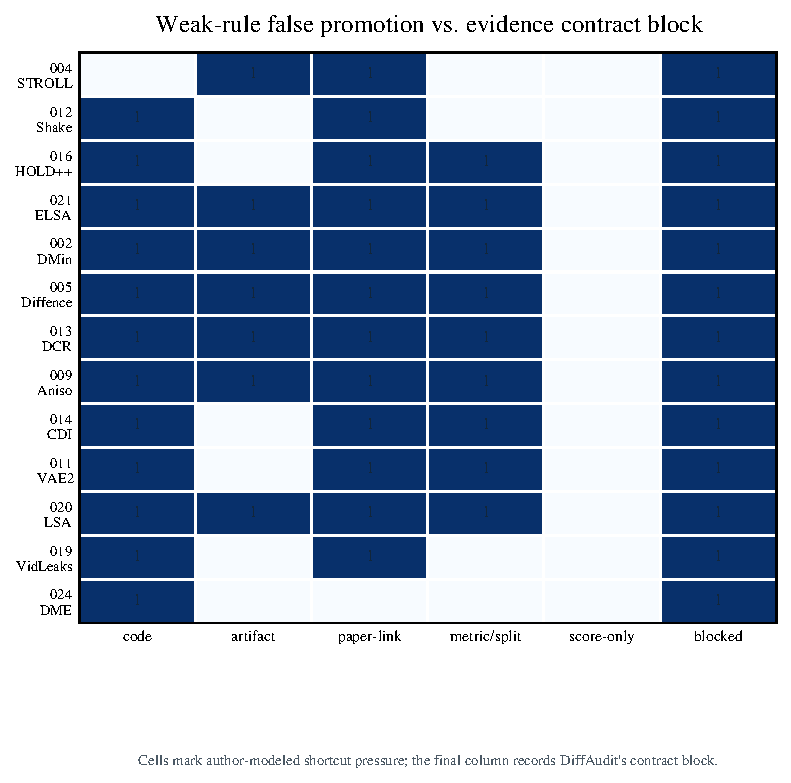
\includegraphics[width=\linewidth]{figures/false_promotion_exemplars.pdf}
\caption{C14 author-keyed stress visualization. Cells mark weak-admission
triggers before reviewer labeling; the final column records the author-keyed
first blocker.}
\label{fig:c14-vis}
\end{figure}

\section{Row-Level First Blocker Records}

The companion packet records the first blocker for each of the 13 selected
rows. A row is non-Pass at the score/response gate when its public surface
lacks row-bound score or response outputs. A row is non-Pass at the
consumer-boundary gate when the target identity, split semantics, or
score provenance cannot be verified from the public surface alone.

All 13 rows are jointly non-Pass at both gates. The purpose of C14 is to
quantify the false-promotion rate that would occur if weak public-surface
rules (code availability, paper-artifact links, metric/split visibility,
artifact availability) were used as admission criteria without the full
6-gate protocol. The observed result---13/13 blocked---confirms that the
contract prevents promotion of metadata-only rows before independent
labeling.

\end{document}
